\chapter{Results}
In this section, the results of the project will be discussed.

\section{System Integration}
This section details the physical system and the integration of the hardware. This inculdes power consumption, system layout, and component failures. The system diagram is shown in Figure \cite{masdr_system_diagram} \par
\begin{figure}[ht!]
	\centering
	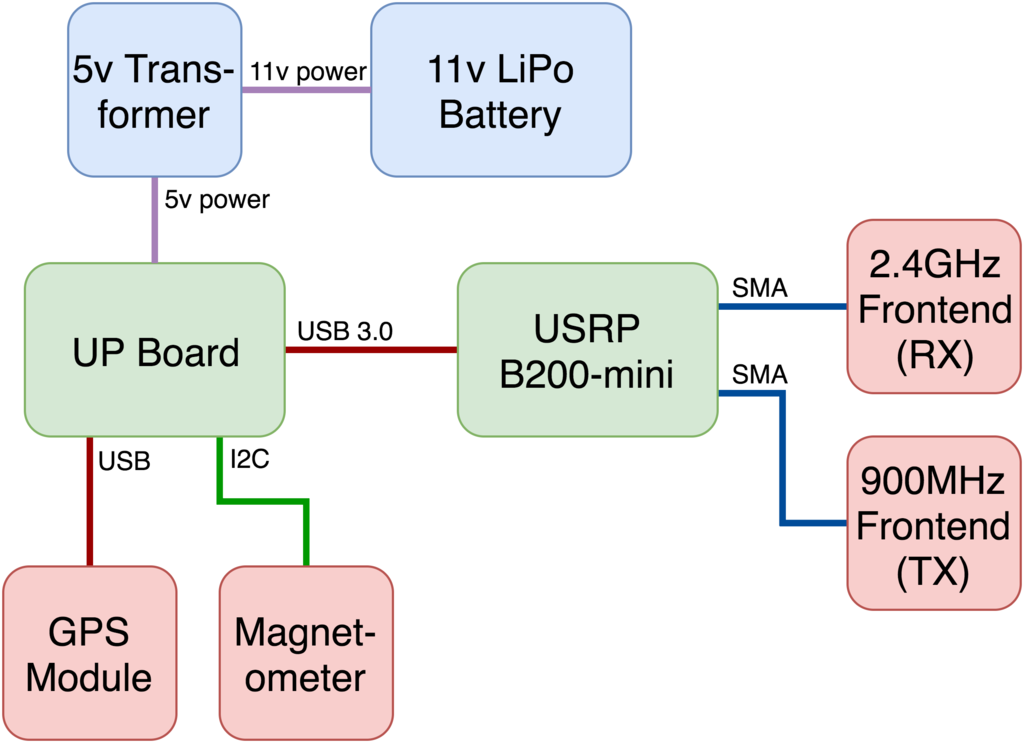
\includegraphics[width=0.70\textwidth]{img/masdr_system_diagram.png}
	\caption{MASDR system diagram detailing the connections between each component.}
	\label{fig:masdr_system_diagram}
\end{figure}\par
To power the system, an 11V LiPo battery was used in combination with a 5V transformer to step down the voltage for use by the UP board. The battery and converter were connected using connectors seen in Figure \ref{fig:connectors}, so that the battery could be disconnected when it is not in use. The male connector was soldered to the transformer and the female connector was soldered to the battery.
\begin{figure}[ht!]
	\centering
	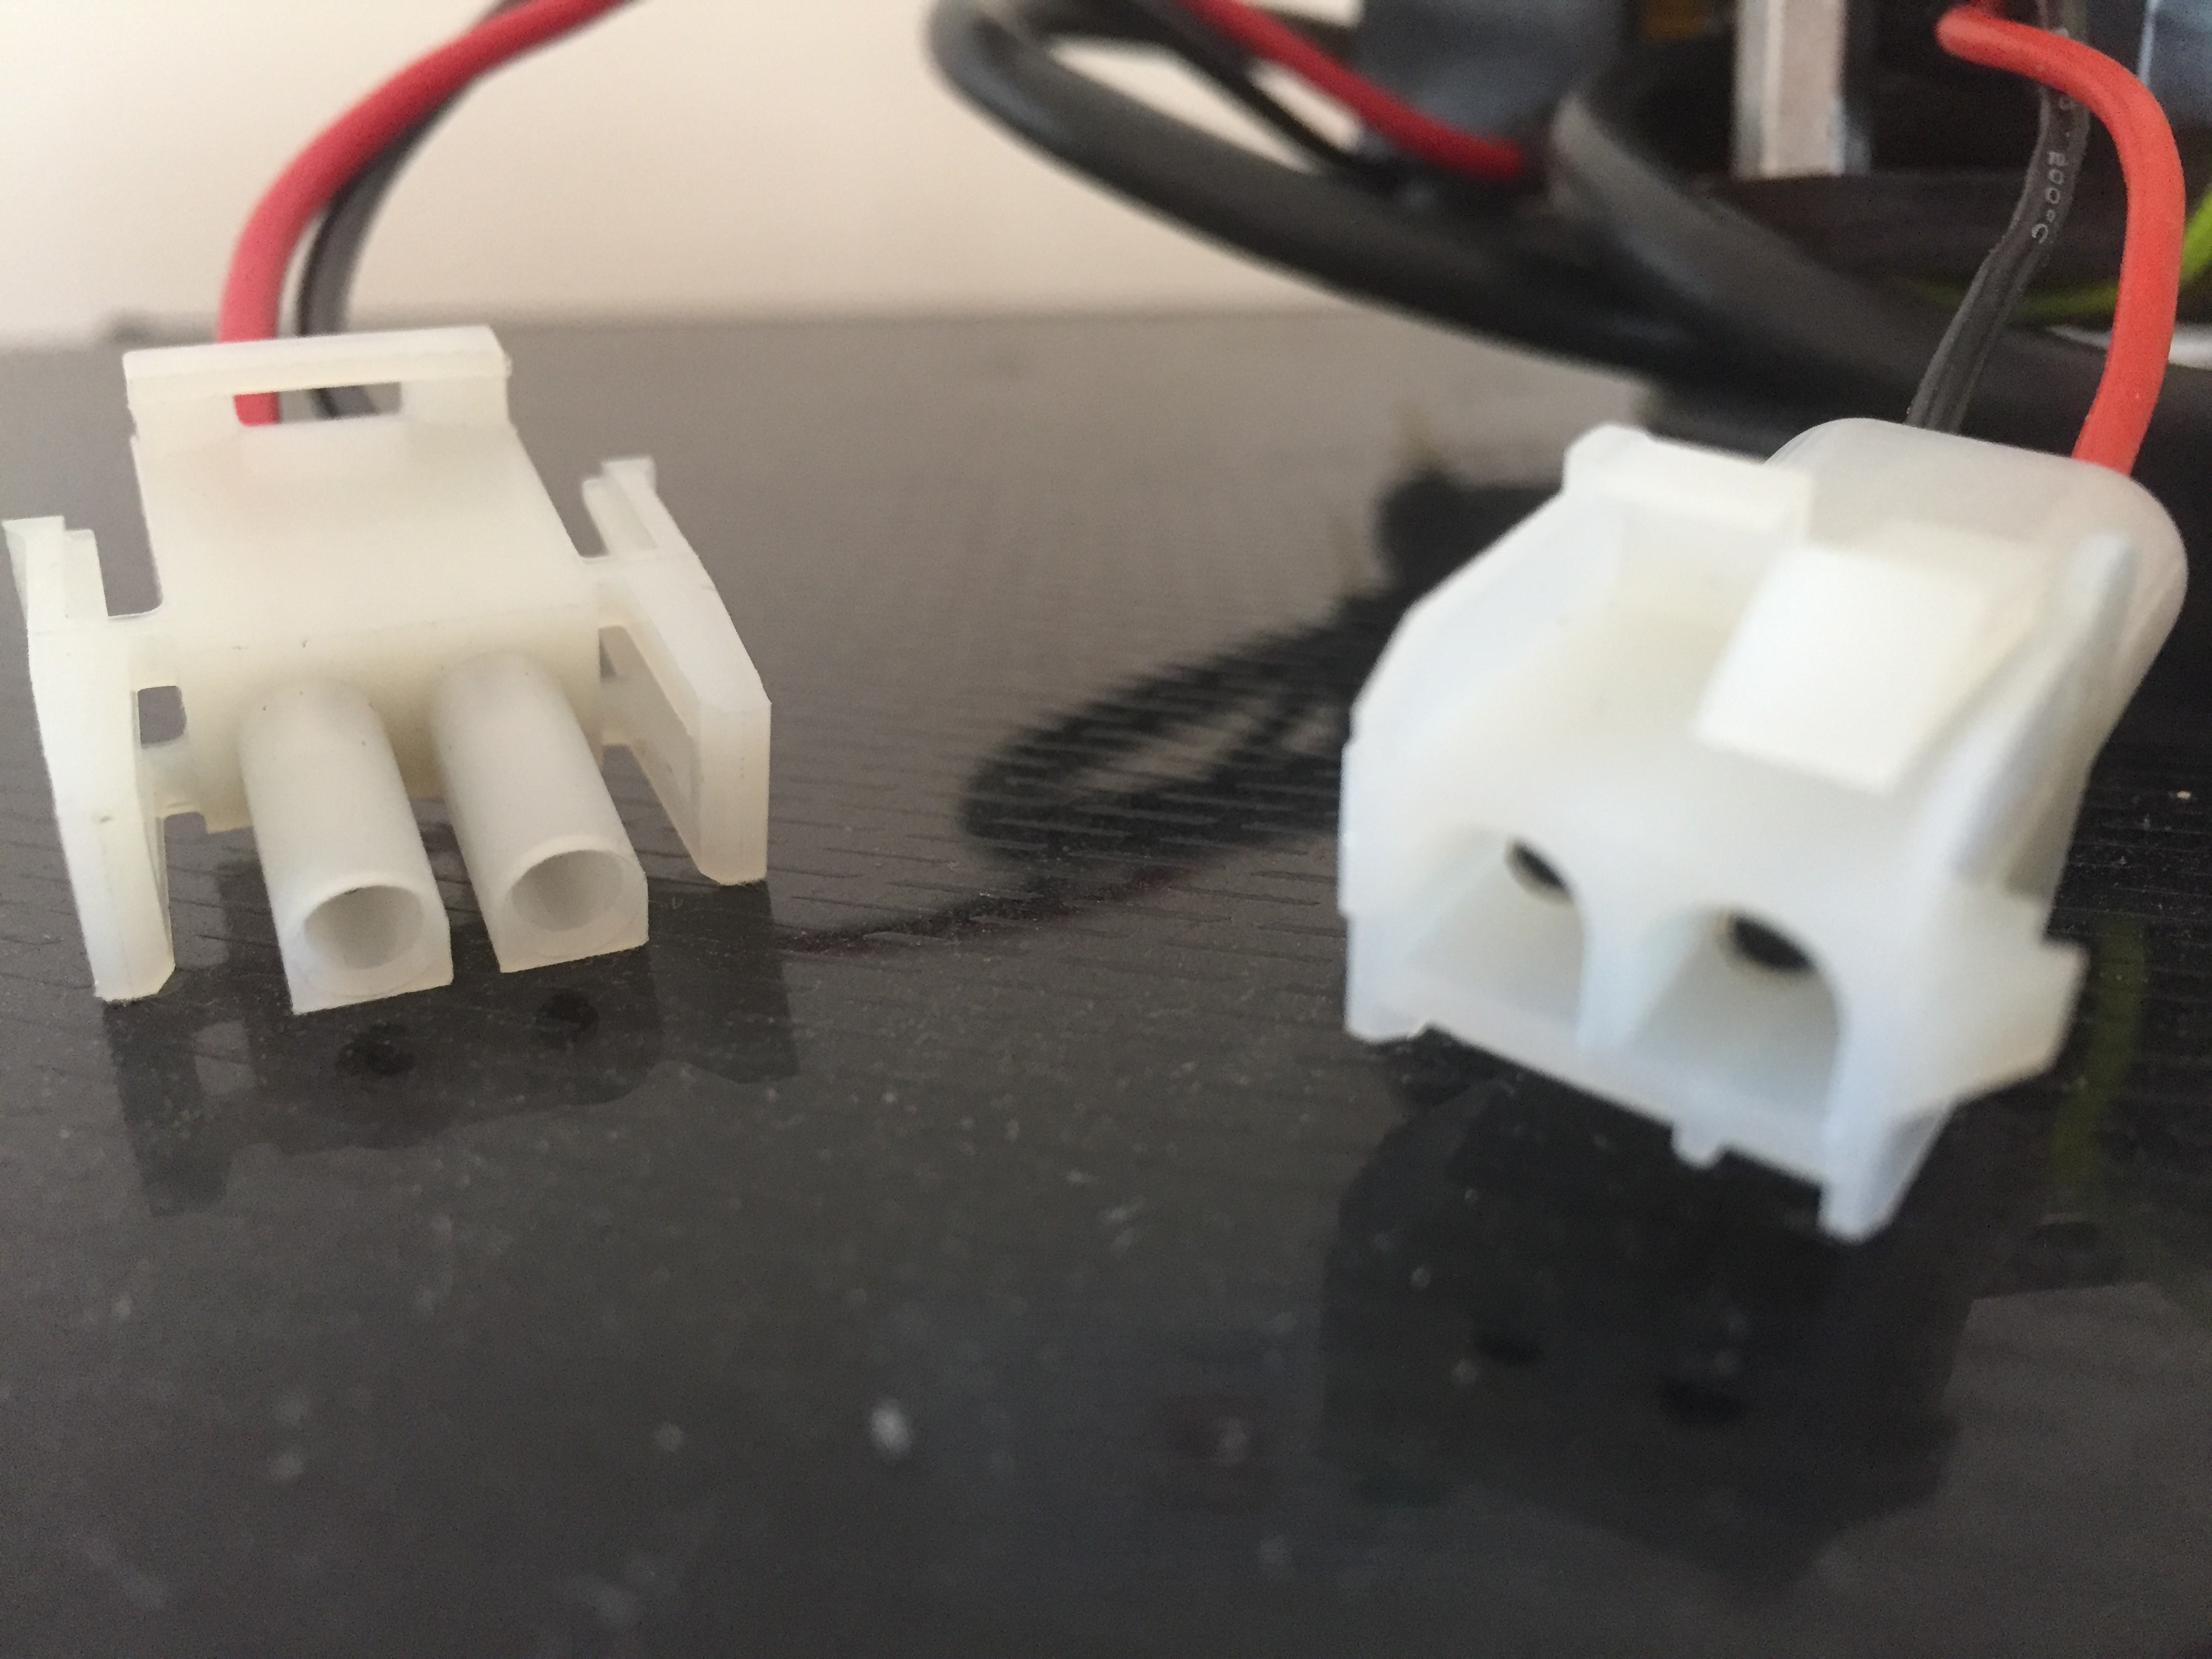
\includegraphics[width=0.70\textwidth]{img/connectors.png}
	\caption{Connectors for the battery. The male connector (left) is connected to the transformer and the female connector (right) is connected to the LiPo battery.}
	\label{fig:connectors}
\end{figure}\par
The first transformer that was used in the sytstem failed because it became disconnected from the UP board when power was applied. Due to the transformer being a _________, which will break when no output is connected. A new tranformer was purchased to replace the malfunctioning one. \par

The encasing for the system was designed in SOLIDWORKS. It was fabricated using wood and a laser cutter. The encasing was designed to be as minimal as possible to reduce the weight of the system. This was done by cutting holes in the wood to remove as much material as possible. Metal supports were used in each of the corners to connect the two wooden sections as seen in Figure \ref{fig:connectors}.
\begin{figure}[ht!]
	\centering
	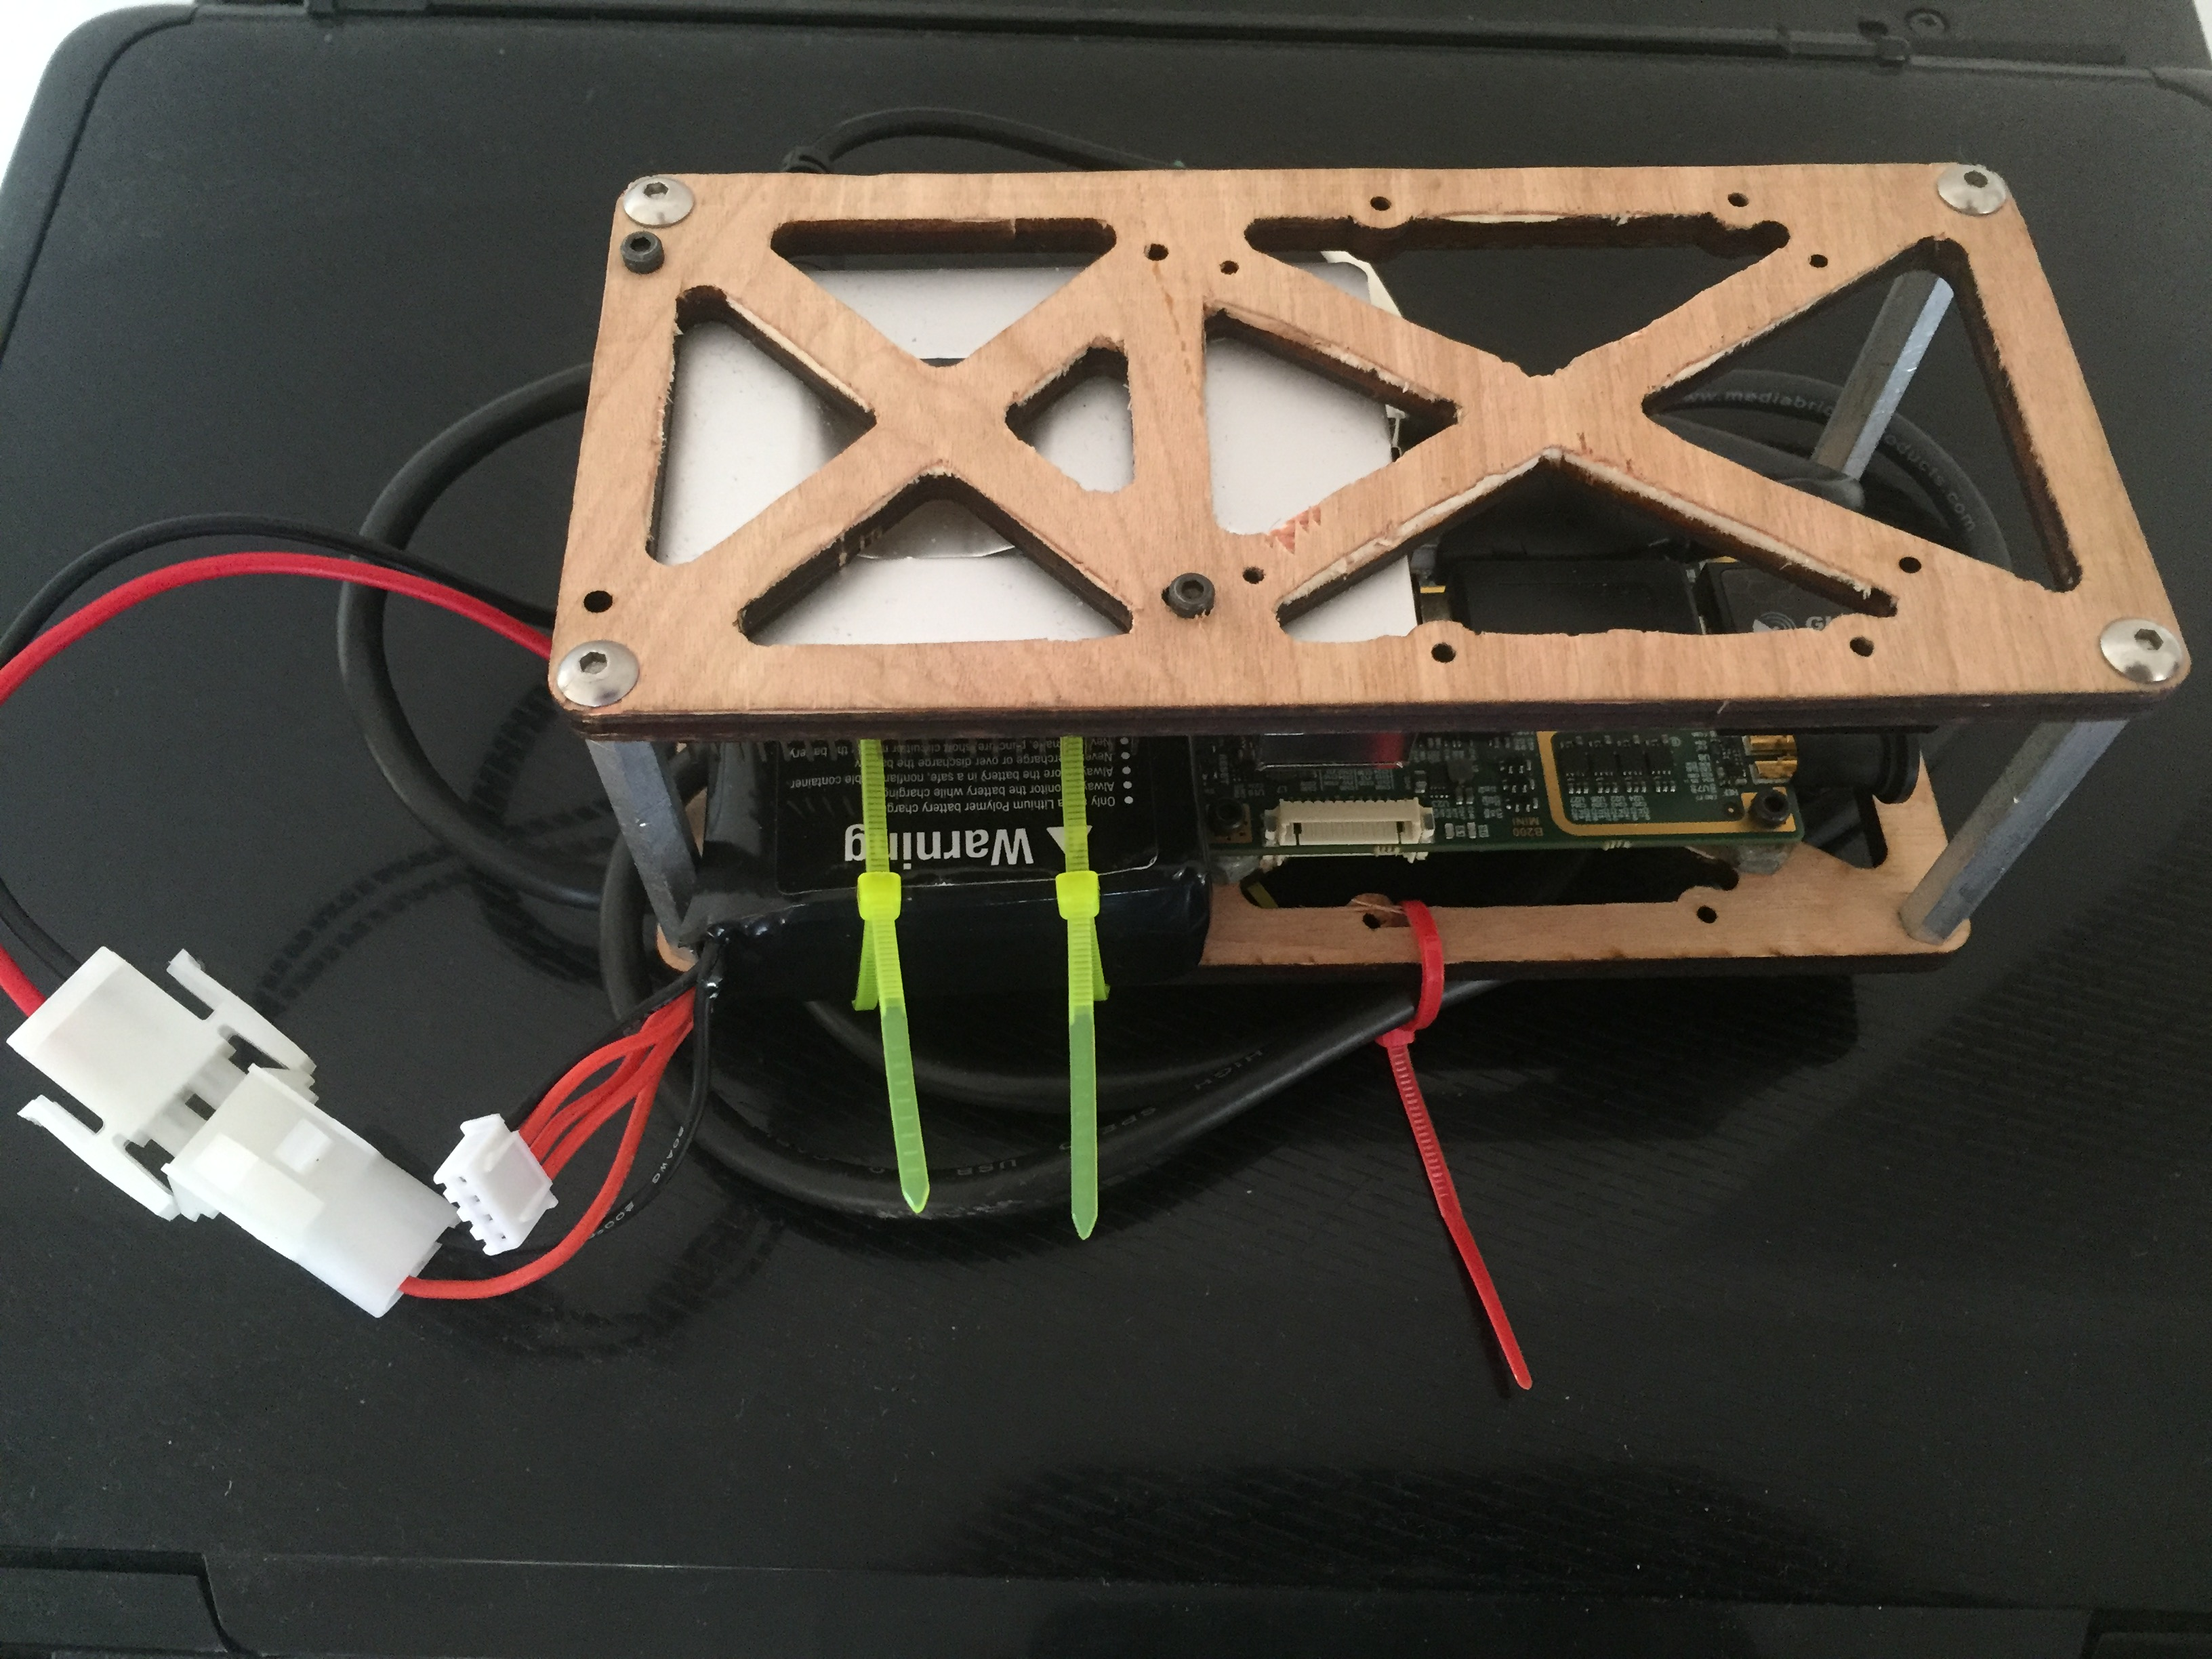
\includegraphics[width=0.70\textwidth]{img/Overhead_of_box.png}
	\caption{Overhead view of the encasing of the MASDR system}
	\label{fig:overhead_of_box}
\end{figure}\par
The two wooden panels were created identically to reduce design time and fabrication time. Screw holes were precut into the wood to ensure mounting the components wouldn't split the wood. This enclosure was mounted to the bottom of the drone using the holes shown in Figure \ref{fig:Solo_mount}. \par


\section{Code Framework}
\section{Drone Control}
\section{Spectrum Sensing}
\section{Spectrum Localization}
\section{Transmit To Ground}
\section{Summary}
